\documentclass[conference]{IEEEtran}
\IEEEoverridecommandlockouts
% The preceding line is only needed to identify funding in the first footnote. If that is unneeded, please comment it out.
\usepackage{cite}
\usepackage{amsmath,amssymb,amsfonts}
\usepackage{algorithmic}
\usepackage{graphicx}
\usepackage{textcomp}
\usepackage{xcolor}
\usepackage{float}
\usepackage[hidelinks]{hyperref}
\def\BibTeX{{\rm B\kern-.05em{\sc i\kern-.025em b}\kern-.08em
    T\kern-.1667em\lower.7ex\hbox{E}\kern-.125emX}}
\begin{document}

\title{Implementation of TrustRank using Pregel Framework}
    \author{\IEEEauthorblockN{Aman Panwar}
    \IEEEauthorblockA{{CS20BTECH11004} \\
    \textit{Department of Computer Science}}
    \\\
    \IEEEauthorblockN{Taha Adeel Mohammed}
    \IEEEauthorblockA{{CS20BTECH11052} \\
    \textit{Department of Computer Science}}
    \and

    \IEEEauthorblockN{Amulya Tallamraju}
    \IEEEauthorblockA{{AI20BTECH11003} \\
    \textit{Department of Aritificial Intelligence}}
    \and

    \IEEEauthorblockN{Pranav K Nayak}
    \IEEEauthorblockA{{ES20BTECH11035} \\
    \textit{Department of Engineering Science}}
    \\

    \IEEEauthorblockN{Vikhyath Sai Kothamasu}
    \IEEEauthorblockA{{CS20BTECH11056} \\
    \textit{Department of Computer Science}}
    }

\maketitle

\section{Introduction}
In this report, we attempt to document our implementation of the TrustRank algorithm by using the Pregel Framework
\section{Problem Statement}

\subsection{TrustRank}
TrustRank is a Search Engine Optimization (SEO) algorithm developed by researchers at Stanford University in 2004. It is designed to combat the manipulation of Search Engine Results Pages by spam websites. These websites will often attempt to trick search engines and boost their positions search results. For example, a commercial website attempting to exploit SEO might populate its homepage with thousands of keywords, allowing it to be pulled up as a result on searches that aren't relevant to the website itself. It can hide this text from users visiting the website by manipulating color schemes and backgrounds. As a result, the web page is displayed as a result for multiple different types of searches.

As another example, search engines will often use the number of incoming links into a web page as a sign that it should be placed higher up in search results. Spammers can then create thousands of bogus web pages, and have links in them that point to the spammer's main web page. This will cause it's rank in the SERP to undeservedly get boosted.

This is where TrustRank comes in. It assigns trust scores to a web page that are used when considering the page's position in a SERP. It does this by assigning a few 'seed' pages, and propagating good scores to those pages that are in proximity to the seed ones.

The algorithm also evaluates the quality of content on a web page, determining if the content on the web page is meets a certain standard. If it does, its score is boosted, while if the content is determined to be substandard, such as spam websites that have multiple links to low score pages, its score is correspondingly lowered.


\subsection{Pregel}
Pregel is a large scale graph processing framework, first publicized in a paper by Google in 2010. It is a framework designed for large scale graph processing. Each Pregel computation consists of a series of iterations, called supersteps. Each superstep consists of a computation phase and a communication phase. In the computation phase, each vertex can perform a computation based on its state and the messages it has received from other vertices. In the communication phase, each vertex can send messages to other vertices. The computation and communication phases are repeated until the algorithm terminates.

Pregel is capable of operating on such large graphs by partitioning the graph into smaller subgraphs, and distributing them across multiple machines. Each machine is responsible for a subset of the vertices and edges of the graph. The machines then communicate with each other to perform the computation.

\section{Description of the dataset}
For this assignment, we were given the same dataset as Assignment 1: Circular Trading detection. It consists of 130,535 rows, each row consisting of three column values. The first two contain IDs for entities within the dataset, with the third column containing a number representing the value of the transaction between them.

We apply TrustRank to this dataset to give scores to all the dealers in the dataset, given a small collection of bad sellers. This score is an indicator of the trust given to each seller by the algorithm, with higher scores indicating less trustworthy sellers.

\section{Algorithm Used}
We implement TrustRank here to allow us to quantify how trustworthy dealers are, given a small collection of dealers we know are bad. This is analogous to how TrustRank is implemented for websites, except while the 'seed' pages for the web are trusted pages with a high score, the 'seed' dealers for our dataset are untrustworthy dealers with a high score. The algorithm then propagates this score to other dealers in the dataset, with the score decreasing as the distance from the seed dealers increases. A lower score thus indicates a more trustworthy dealer.
\subsection{Our Implementation in Detail}
We begin the discussion of our implementation by going over our class structure:
\begin{itemize}
    \item \verb|Vertex|: Represents a single node in the graph. It stores the ID, current score,the adjacency list of its outgoing vertices, a list of incoming weights, and a list of outgoing weights
    \item \verb|Pregel|: Represents a single run of the Pregel system. Contains functionality to run an instance, perform a superstep, partition the vertices, return the ID of the process assigned to a vertex, and check whether vertices are active or not.
    \item \verb|Worker|: A single thread in the Pregel system, responsible for handling a single superstep for a subset of the graph.
    \item \verb|TrustRankVertex|: A TrustRankVertex represents a node in the graph.  It stores its id, its
    current score, and the adjacency list of its outgoing vertices, along with the values incoming into it and outgoing from it during the current superstep. Contains functionality to perform updates on its score from incoming edges.
\end{itemize}
The above are classes that behave as the workhorses of our implementation, performing TrustRank and propagating scores across the graph. We also have a \verb|Graph| class, that represents the graph on which TrustRank acts. We initialize a trust score of $\frac{1}{\text{number of bad nodes}}$ to each of the initial nodes before performing any computations.
We also define the following functions to run TrustRank:
\begin{enumerate}
    \item \verb|pregelTrustRank|: This function runs TrustRank through the Pregel system on our graph. The definition of the function can be found in Figure 1.
    \begin{figure}[H]
        \centering
        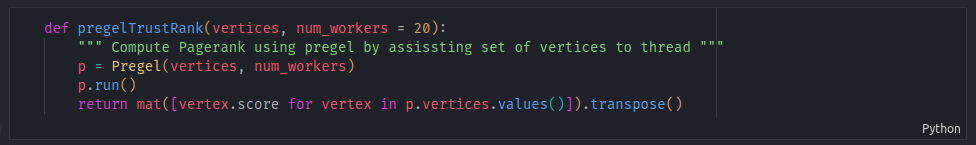
\includegraphics[width=8cm]{images/pregelTrustRank.png}
        \caption{The pregelTrustRank function}
        \label{fig:my_label}
    \end{figure}
    \item \verb|trustrank_test|: This function runs a standard matrix-theory based implementation of TrustRank on our graph for comparison with the Pregel run. The definition of the function can be found in Figure 2.
    \begin{figure}[H]
        \centering
        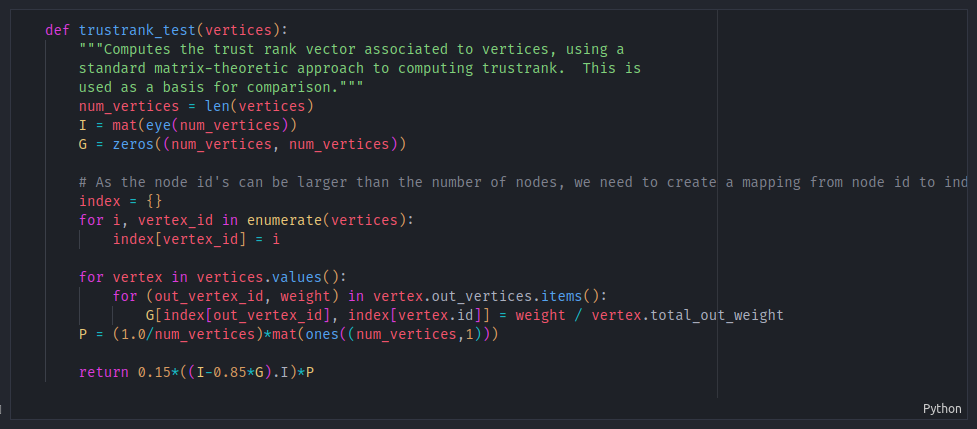
\includegraphics[width=8cm]{images/matrixTrustRank.png}
        \caption{The trustrank\_test function}
        \label{fig:my_label}
    \end{figure}
\end{enumerate}

\section{Results}
We run our \verb|main| function to output the 20 cells with the highest TrustRank score, when using the Pregel based implementation. These 20 are the "worst" nodes in the network. For comparison, we also include the top 20 computed by the matrix-theory based approach, from which one can see that both give identical results.
\begin{figure}[H]
    \centering
    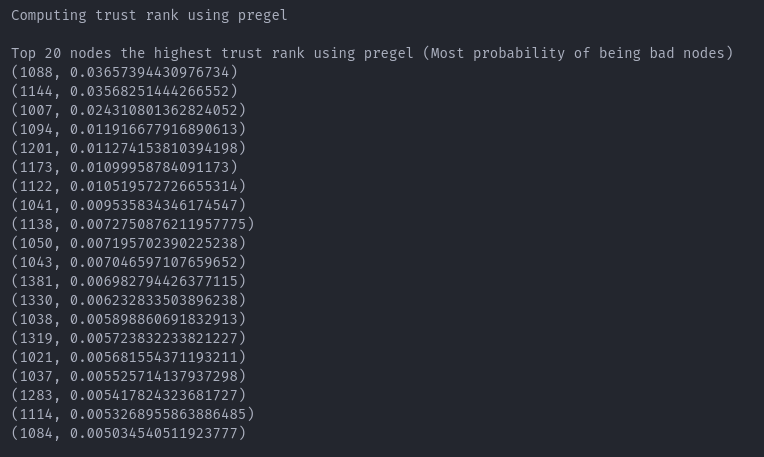
\includegraphics[width=8cm]{images/pregelscores.png}
    \caption{The scores computed by the Pregel based implementation}
    \label{fig:my_label}
\end{figure}

\begin{figure}[H]
    \centering
    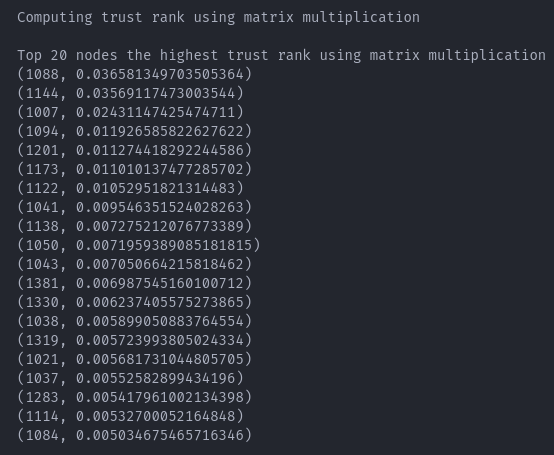
\includegraphics[width=8cm]{images/matrixscores.png}
    \caption{The scores computed by the matrix-theory based implementation}
    \label{fig:my_label}
\end{figure}
While in theory, the Pregel based implementation is supposed to be faster, we observe through noting down the execution times of the notebook's cells that the matrix-theory based implementation is, on average, 8 times faster. We speculate that this is because the overhead of the Pregel system is too large for the small size of our dataset, and the computing power used to manage all the threads is not compensated for. The matrix-theory based approach, while likely inefficient if applied on datasets of the size that Pregel is intended to be used for (i.e. billions of nodes), is much more efficient for our dataset.

In the following figure we have plotted the distribution of the TrustRank scores, on a logarithmic scale.
\begin{figure}[H]
    \centering
    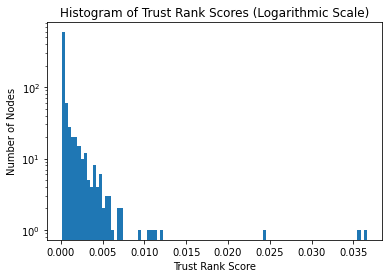
\includegraphics[width=8cm]{images/histogram.png}
    \caption{The distribution of TrustRank scores}
    \label{fig:my_label}
\end{figure}
\vspace{12pt}

\section{References}
\begin{itemize}
    \item \href{https://blog.acolyer.org/2015/05/26/pregel-a-system-for-large-scale-graph-processing/}{Adrian Colyer, "Pregel: A System for Large-Scale Graph Processing}
    \item \href{https://www.vldb.org/conf/2004/RS15P3.PDF}{Gy\"ongyi, Garcia-Molina, Pedersen, "Combating Web Spam with TrustRank"}
\end{itemize}
\end{document}
